\section{Introduction}
\label{Introduction}
%%%What is the purpose of this paper?
%Introducing GCRs here and Victor Hess  - discovery of GCR's : https://sci-hub.tw/10.1038/123155a0
\subsection{Cosmic Rays}
First discovered by Victor F. Hess~\cite{hess}, cosmic radiation penetrates deep into Earth's atmosphere and creates a highly complex radiation environment.  This cosmic radiation is comprised mostly of primary and secondary particles originating from Galactic Cosmic Rays (GCR) and Solar Energetic Particles (SEP). The flux of GCRs, SEPs and their associated secondary particle interactions are affected by various factors such as solar modulation and particle energy.
%Introduce the Solar Cycle and its modulation and how it affects flux of cosmic radiation.
%the solar cycle and GCR flux relationship - the solar cycle is inversely related to GCR flux
In particular, natural variations in the magnetic flux of the Sun - referred to as solar modulation~\cite{abe} influences the intensity of the GCR flux substantially. These natural variations operate on an eleven year cycle known as the solar cycle and are inversely related to GCR flux~\cite{hathaway}. When the sun emits particles in a solar flare or coronal mass ejection, there is an associated increase in the strength of the magnetic field. This magnetic field deflects GCRs away from the Earth, creating a decrease in GCR flux known as a Forbush Decrease~\cite{forbush-decrease}. Consequently, the flux of GCR into the earths atmosphere reaches a maximum during the solar minimum and vice versa.

%Air showers background - sources here: 
%SEP - https://sci-hub.tw/10.1007/978-3-319-50871-9
%SEP and GCR - https://www.ncbi.nlm.nih.gov/pubmed/11542509
As primary particles from SEP and GCR approach the Earth's upper atmosphere, they undergo nuclear interactions.  These interactions produce air showers - cascades of secondary particles that penetrate into the Earth's atmosphere. The distribution of charged particles originating from cosmic rays is not linear and reaches a maximum at a region between \SI{16}{\km} and \SI{18}{\km} referred to as the Regener-Pfotzer Maximum\cite{regener}.
% After some point, the shower maximum, more particles are stopped than created and the number of shower particles declines. Only a small fraction of the particles usually comes down to the ground. 
%Not sure what to do with this statements...
%After reaching peak ionization rates, air showers gradually decrease steadily while decreasing in altitude. 
%After reaching peak ionization rates, the flux of secondary and primary particles decreases steadily while decreasing in altitude.  
%The Regener-Pfotzer Maximum was first discovered by Erich Regener and Georg Pfotzer in 1935~\cite{regener}
%
%%%Suggested Guzik Changes:  Addition to background
%Need more background on the Regener-Pfotzer Maximum - look at main source!
%Need more information regarding primary cosmic rays undergoing nuclear interactions - aka air showers.
%Particles generated peak around 50,000 ft / 15 km.
%Need to mention solar cycle (don't go in-depth though!)  Talk about it and its modulation.
%Solar cycle has 11 year cycle between maximums, and its rotation, magnetic field interactions, and sun spots all affect the radiation environment. 
%Victor Hess - discovery of GCR's : https://sci-hub.tw/10.1038/123155a0
%
%Talk about importance to measure this radiation:
Ionizing radiation at high altitudes has implications to passengers and crew aboard high flying aircraft and astronauts in low earth orbit (LEO), who will absorb a much higher biological dose than they would at the Earth's surface. 
%%%As of 08/26/2019 this ENDS Sam's changes for now - must be reviewed
%The National Council on Radiation Protection and Measurements (NCRP) reported that the average United States citizen receives a radiation dose of about \SI{6.2}{\milli\sievert} per year \cite{ncrp}.
NASA reports that the average person receives an average radiation dose of about \SI{3.6}{\milli\sievert} per year \cite{nasa-dose}, however, this number can be considerably higher if the individual is receiving radiation-based medical treatment \cite{ncrp}.
To provide some context for this number, consider that a crew member aboard the International Space Station (ISS) receives about \SI{160}{\milli\sievert} every six months during solar minimum (when the solar magnetic field provides minimum protection to the crew) \cite{nasa-dose}.
Furthermore, research from the Federal Aviation Administration (FAA) Civil Aerospace Medical Institute has found that passengers and crew on-board a flight from London to Los Angeles will be exposed to an average effective dose of \SI{61.6}{\micro\sievert} \cite{faa}. Exposure to high levels of ionizing radiation increases the risk of cancer and may be linked to other health risks such as increased rate of birth defects and miscarriages \cite{flightatt}. 

NASA has established a standard system to assess the risks for astronauts.
An astronaut's career exposure to ionizing radiation will be limited such that their Risk of Exposure-Induced Death (REID) will not exceed a 3\% chance of cancer mortality \cite{nasa-reid}. The radiation dose that defines this limit is dependent on age and sex, so there is no general number applicable to everyone. Additionally, this standard is not applied to typical radiation workers, who are limited to \SI{50}{\milli\sievert} per year.

%Paper for miscarriages and birth defects
%Another possible source: https://www.ncbi.nlm.nih.gov/pmc/articles/PMC4510952/ and further confirmed by: https://www.cdc.gov/niosh/topics/aircrew/reproductivehealth.html
%s. "For flight attendants, a NIOSH study found that exposure to 0.1 mGy (0.36 mSv) or more of cosmic radiation in the first trimester may be linked to increased risk of miscarriage"
Lastly, data from the CRaTER cosmic ray telescope aboard NASA’s Lunar Reconnaissance Orbiter has shown that dose rate from cosmic rays in the vicinity of the moon has reached the highest level observed since the beginning of the space age \cite{crater}. The health risks associated with exposure to radiation in the atmosphere and in space combined with the increase in cosmic ray intensity during solar minimum periods point towards the necessity of the development of a relatively low cost device for monitoring the radiation environment in real-time.

%%%START As of 08/26/2019
%%Suggested Guzik Changes: We need to include more background on the MiniPIX
%this includes more discussion about our instrument
%include and discuss relevant figures
%include electronic circuits/configuration
%Discuss instrument development
%need general background of instrument (From Renshaw: It was developed by the TimePIX/MiniPIX Collaboration originally and commercialized and sold by Advacam, you should make this point more clear, and then also give a reference to the original Collaboration paper that introduces the devices.
%Talk about minipix works! how we can get dose from the device - there is no derivation from the counts!
%include talk about Clusters and cluster types - 
%%what is a cluster type and why should anyone care (include relevant figures)
%What are LET and Quality Factors and why are they important
%Show it works (this is our raw data!)
%
\begin{figure}[H] %DISCUSS THIS FIGURE AND REFERENCE IN TEXT
    \centering
    %%%%%%%%%%%%%%%change to width=0.35\textwidth for print
    %width=/textwidth for review
    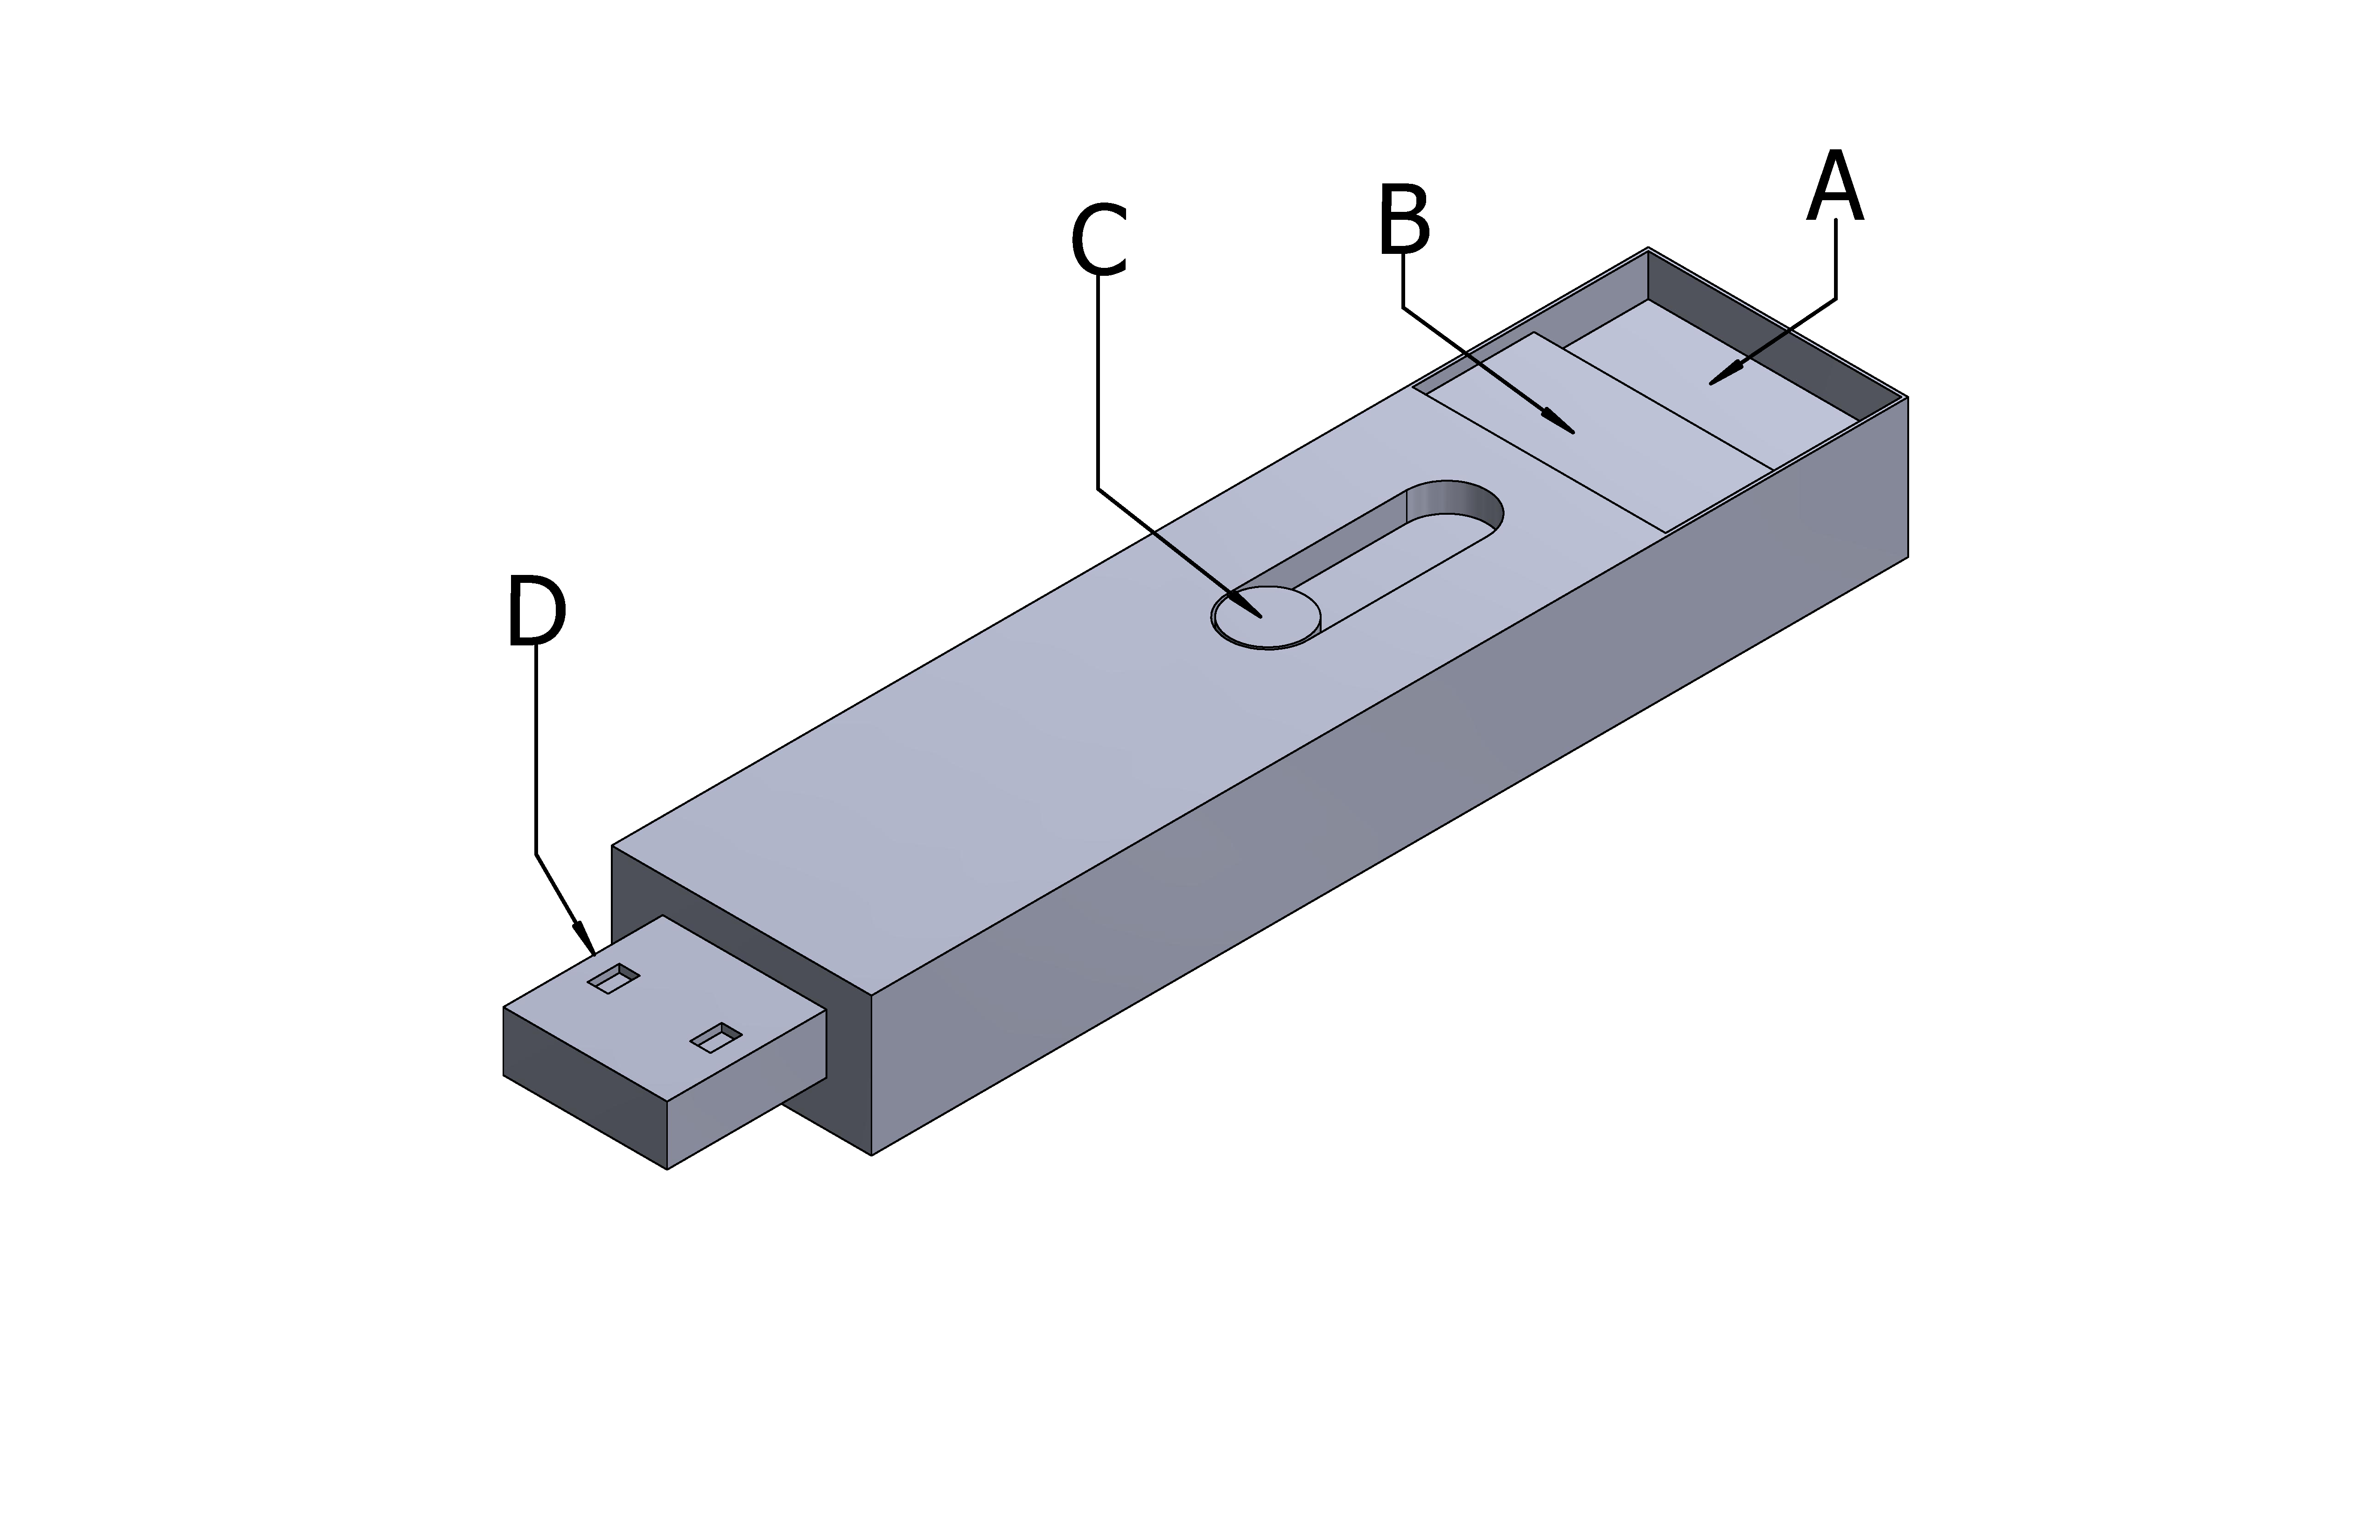
\includegraphics[width=\textwidth]{MiniPIX_Device.pdf} 
    \caption{MiniPIX~\cite{advacam} USB Device. A is the sensor window, B is the protective cover, C is protective cover switch, and D is the USB.}
    \label{fig:minipix_usb}
\end{figure}
%
The MiniPIX, shown in Figure~\ref{fig:minipix_usb}, is a portable radiation camera developed by the TimePIX-MiniPIX Collaboration and commercialized by Advacam~\cite{advacam}.  It utilizes a 256x256 pixel silicon TimePIX Application Specific Integrated Circuit (ASIC) and a USB readout interface. Hybrid pixel sensors, such as the TimePIX ASIC, are made up of two chips connected together via bump bonding. One chip consists of the pixels and the other consists of the read-out electronics for each pixel. Each pixel in the array performs as an individual detector and is a semiconductor sensor with its own associated electronics. The details of the measurement process are given by Ref. \cite{jakubek-pixel-detectors}, but the following is a summary of this process. One component in the pixel's electronics is a semiconductor diode. When incoming ionizing radiation comes into contact with the depleted volume of the diode, the diode generates a charge. This charge is transported using an electric field to electrical contacts where the pixel's read-out electronics can process the information. These electronics perform a signal amplification, discrimination, and an analog-to-digital conversion or counting. Finally, the diode is depleted by a reverse bias, and the process is repeated for the next measurement

The MiniPIX operates in a frame-based data readout mode and has a digital shutter~\cite{stuartthesis}. The device can be operated under one of three modes: time-of-arrival (TOA), time-over-threshold (TOT), or single particle counting.  TOA mode for particle analysis measures the pulse arrival time recorded on the silicon chip.  TOT mode can be used to measure the charge of incident particles onto the detector.  Single particle counting mode counts each pulse once over a given threshold. Frame length varies with each mode and is the main limiting factor for MiniPIX applications.  The built-in counter may be saturated if frame length isn't limited for each mode.  In general, the frame length must be kept short for all modes.  Tracks from single particle events can be measured in TOT mode, therefore frame length must be kept short to prevent tracks from overlapping~\cite{stuartthesis}.  Such tracks can be seen in Figure~\ref{fig:sample_2018}, recorded on the 2018 SORA flight.
%
\begin{figure}[H] %DISCUSS THIS FIGURE AND REFERENCE IN TEXT
    \centering
    %%%%%%%%%%%%%%%change to width=0.35\textwidth for print
    %width=/textwidth for review
    
\includegraphics[width=\textwidth]{2018_track.pdf} 
    \caption{Particle track recorded from 2018 SORA flight}
    \label{fig:sample_2018}
\end{figure}

%%% Guzik recommends we explain what the different modes mean:
%TOA:TOA mode measures the time from when the preamp goes high against the threshold until the end of the acquisition frame.Time of Arrival - measures the arrival time of a pulse. In TOA mode the chip measures the particle arrival time by counting from when the preamplifier goes high on the discriminator to the end of the acquisition (which can be triggered in hardware, or in software).
%
%TOT: The TOT mode in the Timepix ASIC measures the time elapsed while the preamp output is high against the threshold discriminator. • Time Over Threshold (TOT) - charge measurement. In TOT mode whenever the pulse is high against the discriminator the pixel counts until the pulse is low again. This allows each pixel to act as a Wilkinson type ADC measuring the discharge time of the preamplifier (i.e. the time spent over the threshold). The minimum threshold is about 1000 electrons or 3.6keV with a silicon sensor. As each pixel is individually programmable, it is possible to operate different pixels in different modes during the same acquisition.
%
%Single Particle Counting: "MediPIX mode" In Medipix mode the chip counts the number of times the signal goes higher than the threshold. Medipix - photon/pulse counting.
%
%Each pixel in the Timepix contains a preamplifier, discriminator threshold, 14 bit counter and can operate in one of three modes
%
The MiniPIX is capable of individual particle differentiation and when operating in TOT mode can be used to measure dosimetric endpoints such as absorbed dose and dose equivalent. Individual particle tracks are defined as clusters, which are groups of neighboring pixels on the sensor.  Cluster formation along with the measured Linear Energy Transfer (LET) both are use in the analysis of absorbed dose and dose equivalency.
%go in further depth talking about cluster formation
%talk about LET and absorbed dose
%talk again about individual particle differentiation
%introduce image

\begin{figure}[H]
\centering
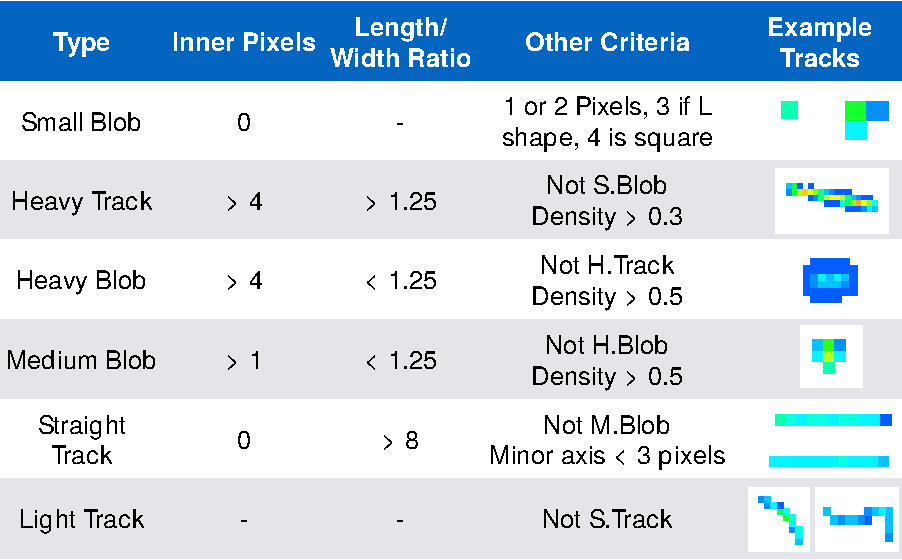
\includegraphics[width=\textwidth]{stuartgraphic.pdf}
\caption{Cluster types\cite{stuartalgo}}
\label{fig:stuartfigure}
\end{figure}

Similar devices to the MiniPIX utilizing a TimePIX ASIC have been evaluated on high altitude balloon flights by Urbar et.al \cite{bexus} and are currently deployed on the ISS for performing real-time space radiation monitoring \cite{timepixiss}. However, the usage of the MiniPIX in combination with a low cost single board computer as a portable radiation monitoring device has yet to be fully explored. The SORA flights in 2017 and 2018 served as a test bed for such a system.

%
%\begin{figure}[H] %DISCUSS THIS FIGURE AND REFERENCE IN TEXT
%    \centering
%    %%%%%%%%%%%%%%%change to width=0.35\textwidth for print
%    %width=/textwidth for review
%    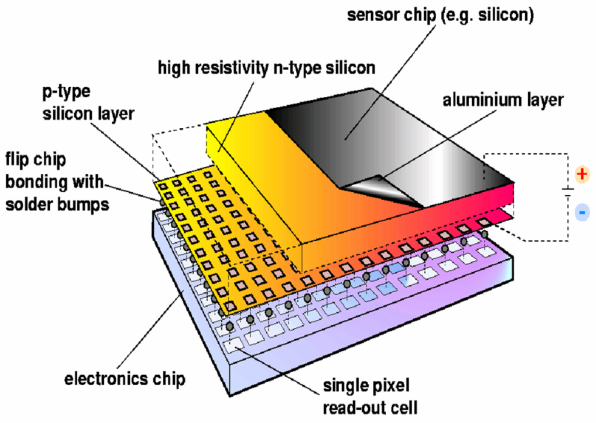
\includegraphics[width=\textwidth]{minipix_silicon.pdf} %REVIEW #1:  May need to find a better image that is not a screen grab.
%    \caption{TimePIX detector structure concept design \cite{TimePIX} }
%    \label{fig:minipix_silicon}
%    %source for image: Measurement of the energy resolution and calibration of hybrid pixel detectors with GaAs:Cr sensor and Timepix readout chip - Scientific Figure on ResearchGate. Available from: https://www.researchgate.net/figure/a-Structure-of-a-Timepix-detector-b-Timepix-pixel-detector-with-USB-interface-FITPix_fig3_270906129 [accessed 23 Apr, 2019]
%\end{figure}
%%

During the High Altitude Student Platform (HASP) 2017 and 2018 flights \cite{hasp}, the SORA payloads carried a MiniPIX interfaced with a Raspberry Pi 3 B+ (RPI) Single Board Computer~\cite{rpi} to test the feasibility of a system for real-time measurements of absorbed dose from cosmic radiation. Data, such as counts and absorbed dose from the MiniPIX, was downlinked and analyzed in real time through the HASP downlink interface. 
%We need to add:
%Electronic circuits of our payload - if possible
%Instrument development details for each mission (not the settings, just the development that went into it)
%More background if necessary of how the MiniPIX works

The HASP 2017 flight launched from Fort Sumner, New Mexico on September 4th, 2017 at 14:04 UTC and ascended to a float altitude of approximately $\SI{31.5}{\kilo\meter}$ at 16:22 UTC; which was maintained for approximately \SI{10.5}{\hour}. The HASP 2017 payload drifted west for a total ground distance of \SI{580}{\kilo\meter} and was recovered just north of the Apache-Sitgreaves National Forest in Arizona.  On September 4th, 2018 at 14:03 UTC the HASP 2018 mission launched from Fort Sumner, Mew Mexico.  The 2018 payload reached a stable float altitude of $\SI{37.2}{\kilo\meter}$ at 16:30 UTC and the total float duration was approximately \SI{9.0}{\hour}. The 2018 payload terminated its flight and landed approximately \SI{96.6}{\kilo\meter} southwest of Mt Graham, Arizona after traveling a total distance of \SI{550}{\kilo\meter}.

%START Guzik Changes:
% We need to 1. Setup what is being measured
%2. why its being measured
%3. How comparisons are made
